
\subsubsection{07.10.14}

\begin{enumerate}
	\item The time of beginning and ending of the congregation:
	17:00 - 21:30
	\item Purposes of the congregation:
	\begin{enumerate}
	  \item Write a program to control the robot by joystick.
	  
	  \item Begin to create lift.
	  
    \end{enumerate}
	\item Work, that has been done:
	\begin{enumerate}
	  \item Today was sold control of the robot by joystick. Motor control was carried out using the left analog sensor. During the tests it was found that when a small current is supplied on motors, it can not be rotated, and a loud unpleasant sound, credible evidence that they work for wear. In this regard, it was decided to put a limit on the supply of motors too weak signal.
      
      \item  In order to raise the basket to 120 cm, it was decided to collect two guides, each of which consists of four rails of furniture: two by 30 cm and two by 35 cm. Thus, the working height was 130 cm. The guides were installed on the robot.
      
      \begin{figure}[H]
      	\begin{minipage}[h]{0.31\linewidth}
      		\center{\includegraphics[scale=0.25]{days/07.10.14/images/01}}
      	\end{minipage}
      	\hfill
      	\begin{minipage}[h]{0.31\linewidth}
      		\center{\includegraphics[scale=0.2]{days/07.10.14/images/02}}
      	\end{minipage}
      	\hfill
      	\begin{minipage}[h]{0.31\linewidth}
      		\center{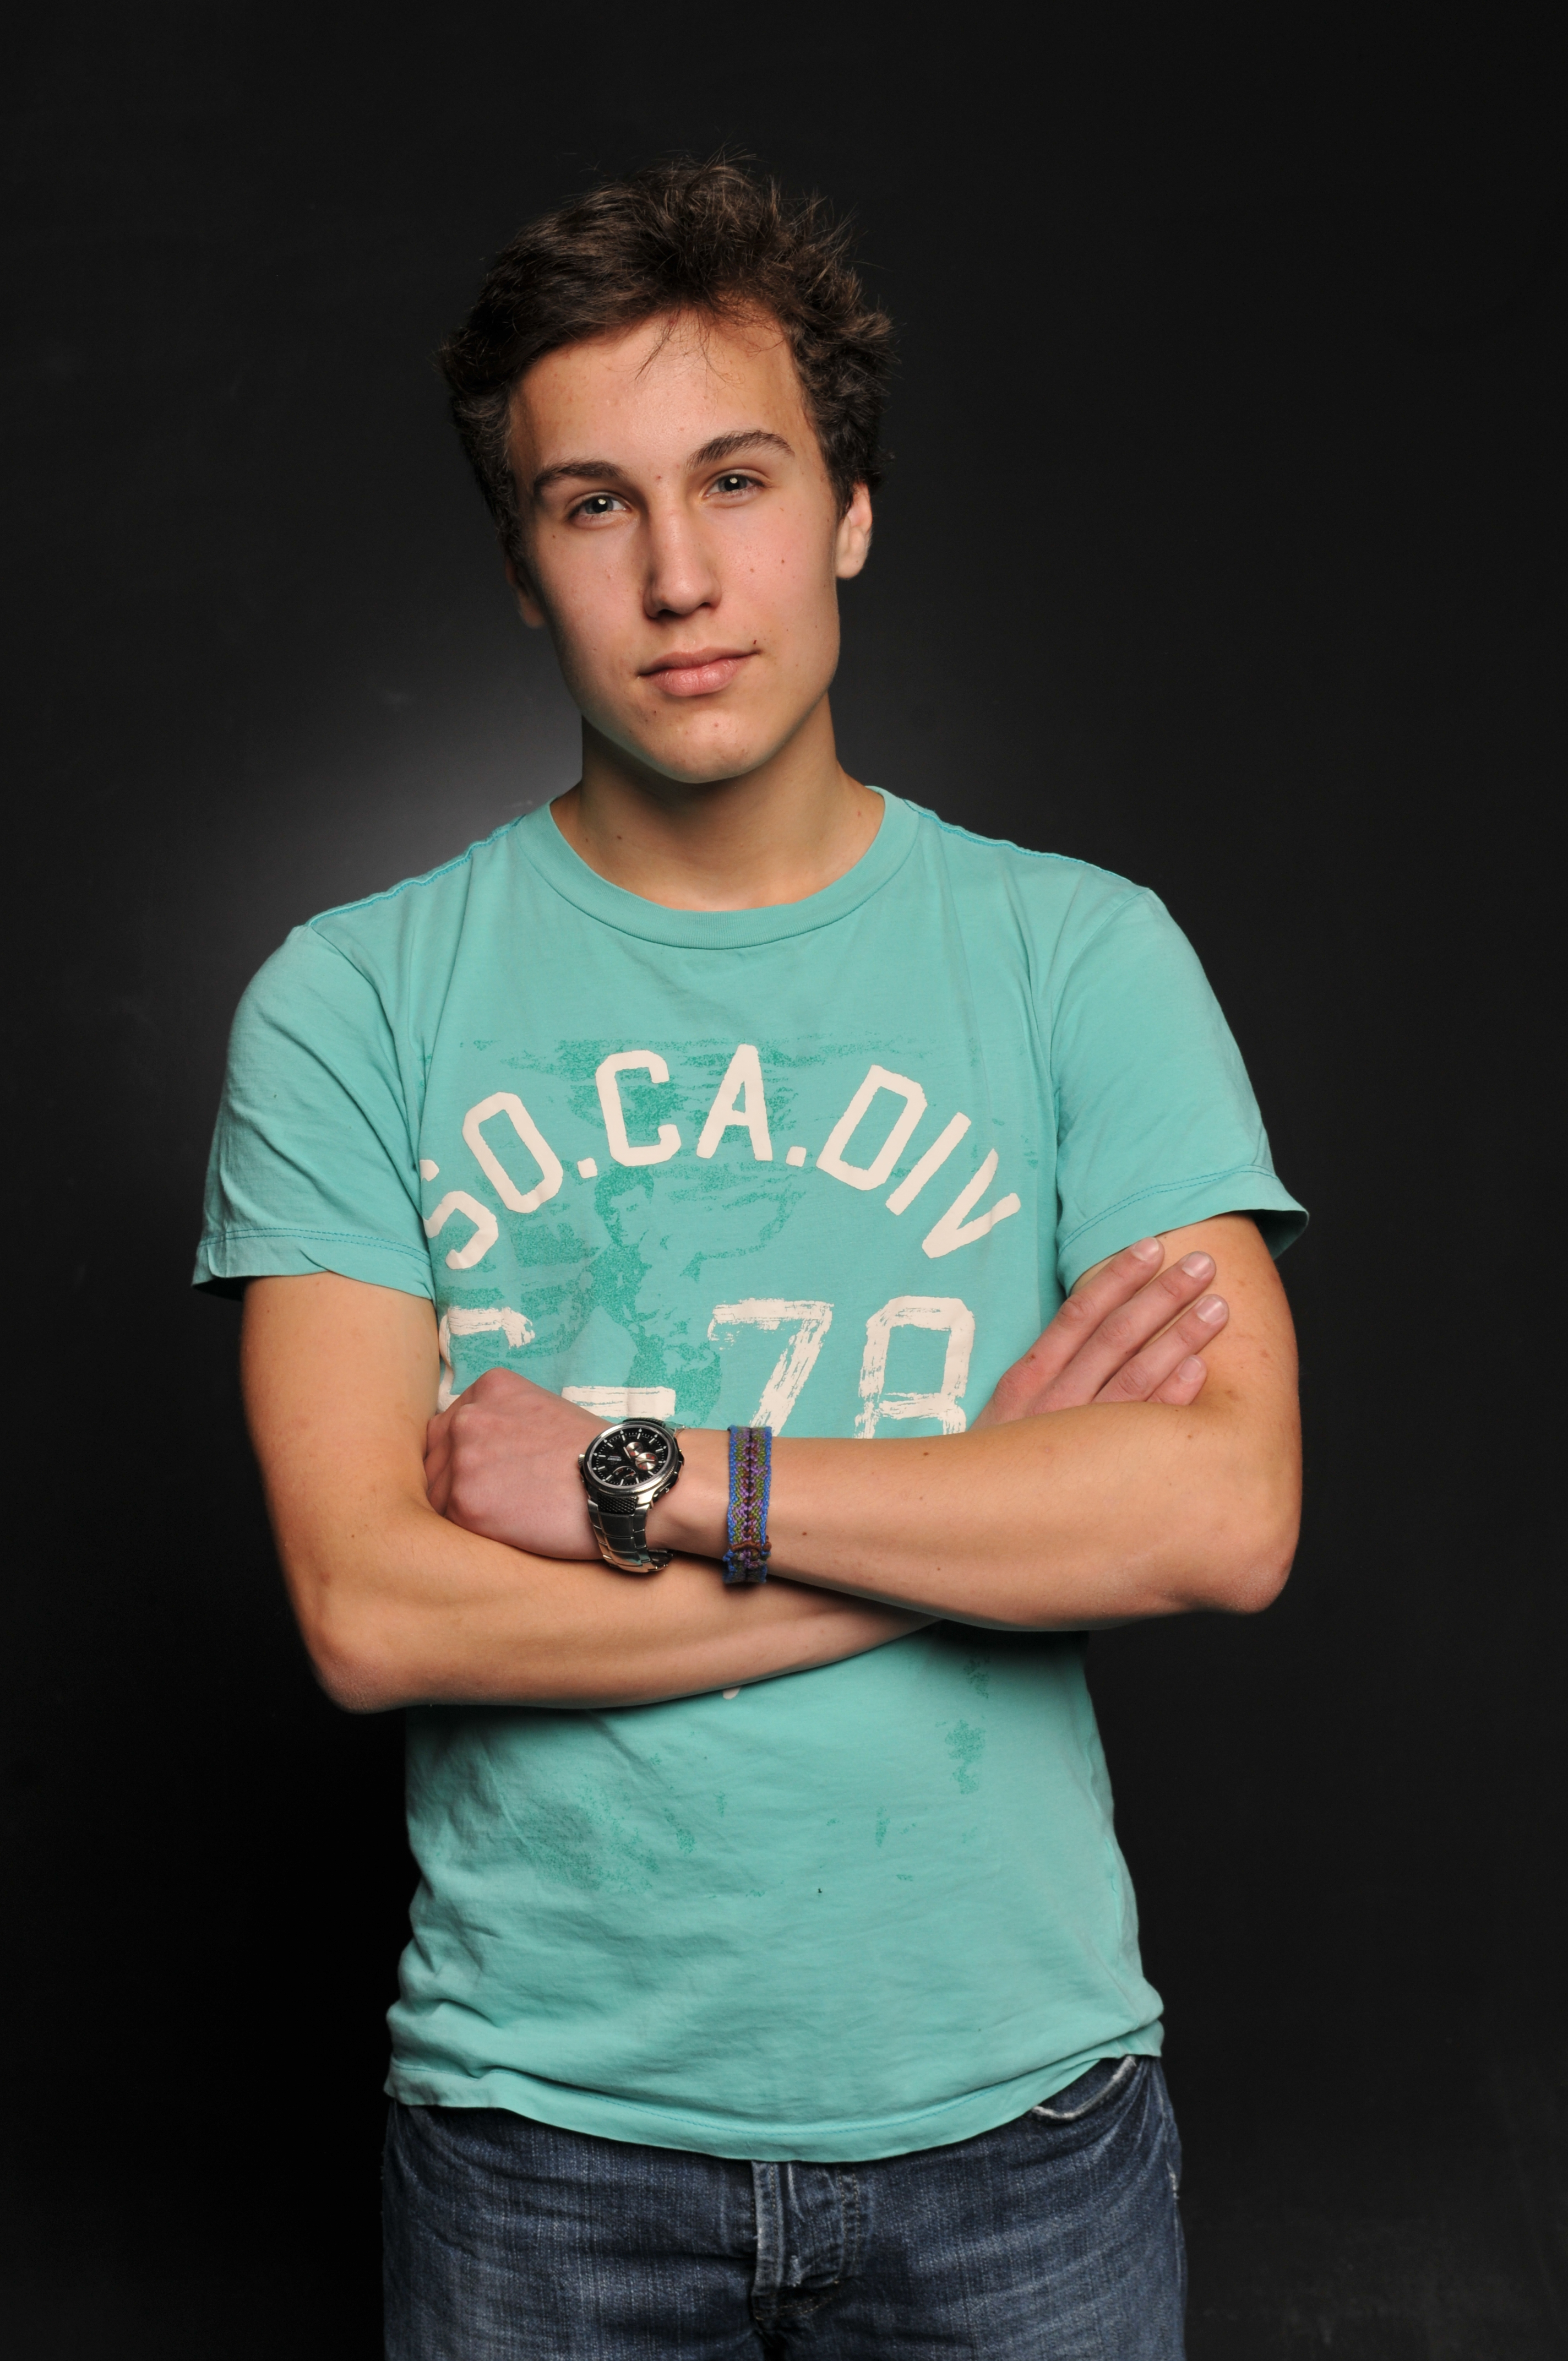
\includegraphics[scale=0.25]{days/07.10.14/images/03}}
      	\end{minipage}
      	\caption{Guides for the lift}
      \end{figure}
      
      \item Because of the internal parts of the robot was much space, it was decided to install a lift in the central part of the robot and electronics in the rear part and secure it there to prevent it from damaging the lifting mechanism disposed adjacent balls. In front of the robot space was left for the bucket. 
       
      \item Because of bucket is lowered inside the robot, it will be protected from collisions with other robots. But in this case, the question arises on how the balls will fall into the bucket, if it will be located inside the robot. To solve this problem, it was decided to increase the distance between the floor and the bottom of the front frame of beam to 7 cm, so that it could go a big ball. This has been achieved by turning the motor around its axis in the field of their mounting position in which the shaft is in the top position to position, in which the shaft is located laterally. In addition, the decision to delay the wheels from each other, increasing the stability of the robot.
      
      \begin{figure}[H]
      	\begin{minipage}[h]{1\linewidth}
      		\center{\includegraphics[scale=0.3]{days/07.10.14/images/04}}
      		\caption{Increase clearance} 
      	\end{minipage}
      \end{figure}
        
      \item Subsequently, in front of the robot, it was decided to establish a soft brush, such as those installed on the snow machines that will rotate and capture balls. In the case when the robot has collected a maximum number of balls, the operator can stop the rotation of the brushes to other balls will not accidentally fall into the bucket.
      
      \begin{figure}[H]
      	\begin{minipage}[h]{0.47\linewidth}
      	    \center{\includegraphics[scale=0.3]{days/07.10.14/images/05}}
      	\end{minipage}
      	\hfill
      	\begin{minipage}[h]{0.47\linewidth}
      		\center{\includegraphics[scale=0.2]{days/07.10.14/images/06}}
      	\end{minipage}
      	\vfill
      	\begin{minipage}[h]{0.47\linewidth}
      	  \center appearance
        \end{minipage}
        \hfill
      	\begin{minipage}[h]{0.47\linewidth}
      	  \center The principle of operation
        \end{minipage}
      	\caption{The idea to capture balls}
      \end{figure}
      
    \end{enumerate}
    
	\item Results:  
	\begin{enumerate}
	  \item  Implement a simple program to control the robot.
	  
      \item  Created and assigned rails for the lift.
      
      \item  Battery and motor drivers are properly fixed on the robot. NXT block has not been fixed, as it requirs periodically to removed for battery replacement.
      
      \item  Clearance of the robot has been increased.
      
    \end{enumerate}
    
	\item Tasks for the next congregations:
	\begin{enumerate}
	  \item Finalize the program of the robot control.
	  
	  \item Implement control of the robot by Bluetooth.
	  
	  \item Create a mechanism for moving apart guides.
	  
    \end{enumerate}     
\end{enumerate}
\fillpage
